\documentclass{article}
\usepackage{graphicx} % Required for inserting images
\usepackage{amsmath}
\usepackage{float} 
\usepackage{listings}
\usepackage{geometry}
\usepackage{makecell}
\usepackage{color}

\geometry{a4paper,scale=0.75}

\usepackage{listings}
\usepackage{xcolor}
\definecolor{mygreen}{rgb}{0,0.6,0}
\definecolor{mygray}{rgb}{0.5,0.5,0.5}
\definecolor{mymauve}{rgb}{0.58,0,0.82}

\lstset{ %
  backgroundcolor=\color{white},   % choose the background color; you must add \usepackage{color} or \usepackage{xcolor}
  basicstyle=\footnotesize,        % the size of the fonts that are used for the code
  breakatwhitespace=false,         % sets if automatic breaks should only happen at whitespace
  breaklines=true,                 % sets automatic line breaking
  captionpos=bl,                    % sets the caption-position to bottom
  commentstyle=\color{mygreen},    % comment style
  %deletekeywords={...},            % if you want to delete keywords from the given language
  %escapeinside={\%*}{*)},          % if you want to add LaTeX within your code
  extendedchars=true,              % lets you use non-ASCII characters; for 8-bits encodings only, does not work with UTF-8
  frame=single,                    % adds a frame around the code
  keepspaces=true,                 % keeps spaces in text, useful for keeping indentation of code (possibly needs columns=flexible)
  keywordstyle=\color{blue},       % keyword style
  %language=Python,                 % the language of the code
  %morekeywords={*,...},            % if you want to add more keywords to the set
  numbers=left,                    % where to put the line-numbers; possible values are (none, left, right)
  numbersep=5pt,                   % how far the line-numbers are from the code
  numberstyle=\tiny\color{mygray}, % the style that is used for the line-numbers
  rulecolor=\color{black},         % if not set, the frame-color may be changed on line-breaks within not-black text (e.g. comments (green here))
  showspaces=false,                % show spaces everywhere adding particular underscores; it overrides 'showstringspaces'
  showstringspaces=false,          % underline spaces within strings only
  showtabs=false,                  % show tabs within strings adding particular underscores
  stepnumber=1,                    % the step between two line-numbers. If it's 1, each line will be numbered
  stringstyle=\color{orange},     % string literal style
  tabsize=2,                       % sets default tabsize to 2 spaces
  %title=myPython.py                   % show the filename of files included with \lstinputlisting; also try caption instead of title
}


\title{\textbf{PDM - Assignment1\\}  Graph Search}
\author{Xiaotong Li\qquad 5965373}
\date{November 2023}

\begin{document}
    
    \begin{titlepage}
        \maketitle
    \end{titlepage}
    
    \tableofcontents
    \newpage

    \setlength{\parskip}{1em}
    
    \section{Graph Search}
    Consider a directed graph $G = (V, E)$, with distances $d(e)$ for each $e \in E$, and consider two nodes $s, t \in V$. For each node $v$ we define the function $P_s(v)$, which gives the length of the shortest path from $s$ to $v$. Similar we define the function $P_t(v)$, which gives the length of the shortest path from $v$ to $t$.
        \subsection{Question1.1}
        Show that for every edge $e = (u, v)$, the length of the shortest path from node $s$ to node $t$ that uses the edge $e$ is $P_s(u) + d(e) + P_t(v)$.

        \noindent
        Answer: Since $G$ is a directed graph, so if you want to get to node $t$ via edge $e=(u,v)$ from node $s$, you must first get to node $u$ from node $s$, then get to node $t$ from node $v$. Since $d(e)$ is fixed, it is obvious that the shortest path from $s$ to $t$ is $P_s(u) + d(e) + P_t(v)$.
        \begin{figure}[H]
            \centering
            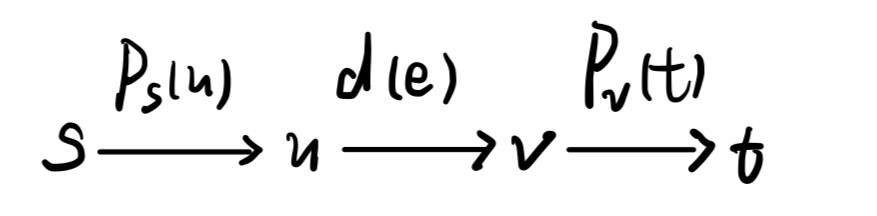
\includegraphics[width=0.5\linewidth]{img1.jpeg}
            \caption{Shortest path from $s$ to $t$}
            \label{1}
        \end{figure}
        \subsection{Question1.2}
        Let $Q$ be the shortest path between the nodes $s$ and $t$. Use the property obtained in Question 1.1, to propose an algorithm that finds the second shortest path from $s$ to $t$ (i.e., considering all paths that are not exactly equal to $Q$)

        \noindent
        Answer: My algorithm is as follows: we choose an edge which is not in the path $Q$, and then we use the algorithm in Question 1.1 to find the shortest path from $s$ to $t$ that uses the edge we choose. We do this for all edges which are not in the path $Q$, and then we can get all the shortest paths from $s$ to $t$ that are not exactly equal to $Q$. Finally, we choose the shortest path from all the paths we get, and this is the second shortest path from $s$ to $t$. The pseudo-code is as follows:
        \newline

        \begin{lstlisting}[language=Python,title={Example code of the algorithm in Question 1.2}]
def second_shortest_path(s, t, Q):
    shortest_path = []
    for edge in E:
        if edge not in Q:
            shortest_path.append(P_s(edge.start) + d(edge) + P_t(edge.end))
    return min(shortest_path)
        \end{lstlisting}
    \newpage
    
    \section{Map to Graph}
    In most cases a graph to operate on is not provided directly. It needs to be extracted from an environment or map first. Use the given map, shown below, to find the \textbf{shortest-path roadmap} that can be used to find the shortest path from the indicated start to the goal location. Obstacles are shown in blue. Also connect the start and goal to the roadmap. Solve this problem graphically. Use the given obstacle sizes and distances to determine the costs of seven edges of your choice.

    \begin{figure}[H]
        \centering
        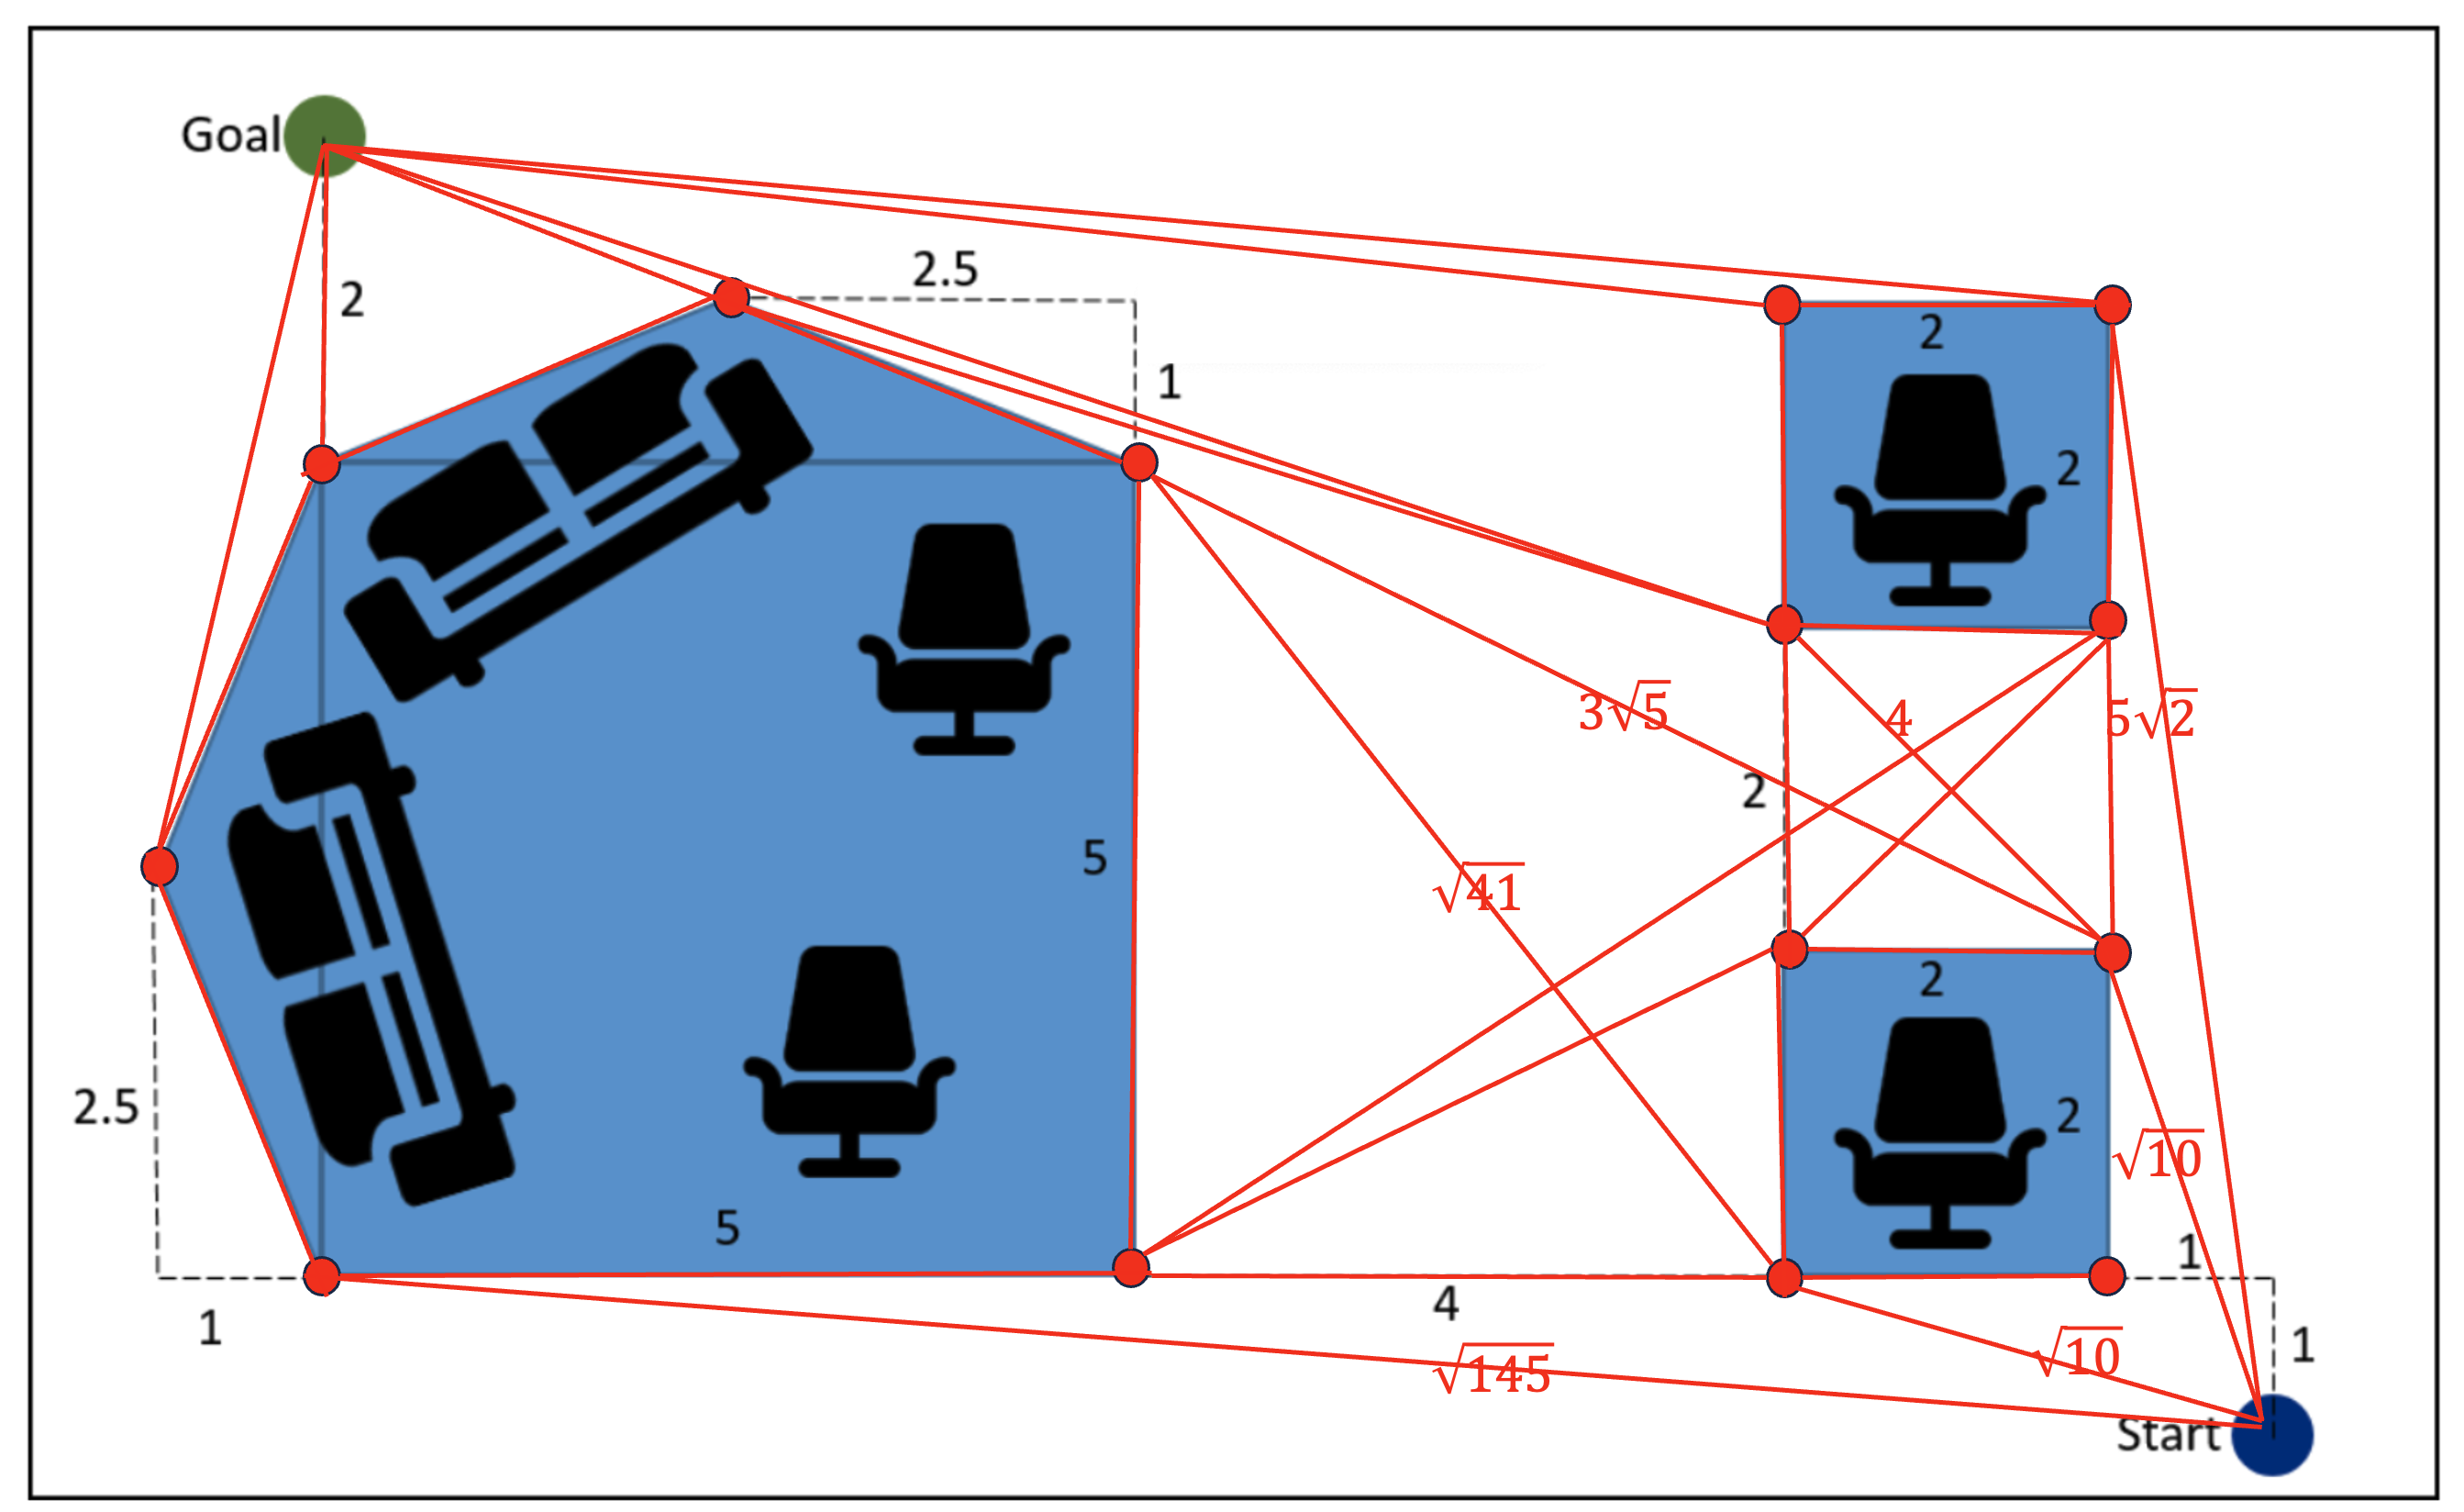
\includegraphics[width=1\linewidth]{img2.jpeg}
        \caption{Graph of roadmap}
        \label{2}
    \end{figure}
    \newpage
    
    \section{Dijkstra and A*}
        Given an environment of operating drones a graph was extracted, similar to the previous exercise. The directed graph avoids collisions with all drones. The cost to traverse an edge is proportional to the distance of nodes and is indicated at each respective edge.
        \begin{figure}[H]
            \centering
            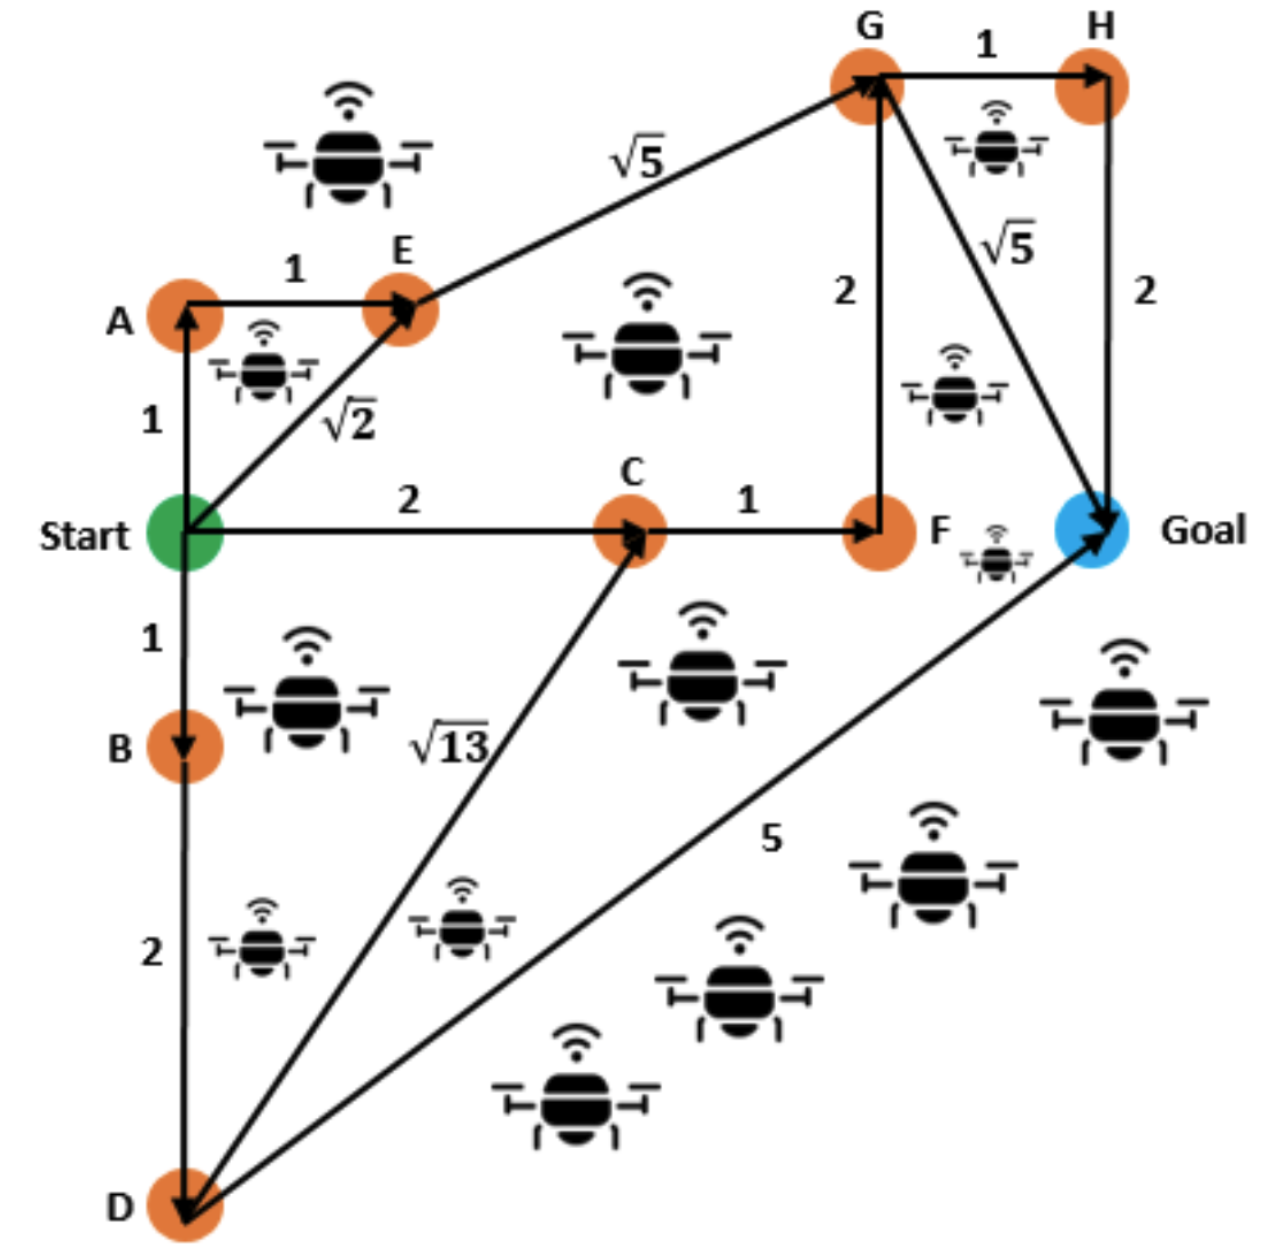
\includegraphics[width=1\linewidth]{img3.jpeg}
            \caption{Graph of environment of operating drones}
            \label{3}
        \end{figure}
        \subsection{Question3.1}
        Find a path form the ”start”-node to the ”goal”-node using the Dijkstra algorithm. Explain each step.

        \begin{table}[H]
            \centering
            \begin{tabular}{c|c|c}
                 Expanded & Q & Explaination\\
                 \hline
                 Start & \makecell*[c]{A(Start,1), E(Start,$\sqrt{2}$),\\ C(Start,2), B(Start,1)} & Explore ABCE from Start \\
                 \hline
                 \textcolor[rgb]{1,0,0}{Start}$\rightarrow$A & E(Start,$\sqrt{2}$), C(Start,2), B(Start,1) & \makecell*[c]{Add A(shortest) to the queue,\\ no new node can be explored from A}\\
                 \hline
                 Start$\rightarrow$A$\rightarrow$B & \textcolor[rgb]{1,0,0}{E(Start,$\sqrt{2}$)}, C(Start,2), D(B,3) & \makecell*[c]{Add B(shortest) to the queue\\ and explore D from B} \\
                \hline
                \makecell*[c]{Start$\rightarrow$A$\rightarrow$B\\$\rightarrow$E} & C(Start,2), D(B,3), G(E,$\sqrt{2}+\sqrt{5}$) & \makecell*[c]{Add E(shortest) to the queue\\ and explore G from E}\\
                \hline
                \makecell*[c]{Start$\rightarrow$A$\rightarrow$B\\$\rightarrow$E$\rightarrow$C} & F(C,3), D(B,3), G(E,$\sqrt{2}+\sqrt{5}$) & \makecell*[c]{Add C(shortest) to the queue\\ and explore F from C}\\
                \hline
                \makecell*[c]{Start$\rightarrow$A$\rightarrow$B\\$\rightarrow$\textcolor[rgb]{1,0,0}{E}$\rightarrow$C$\rightarrow$F} & D(B,3), G(E,$\sqrt{2}+\sqrt{5}$) & \makecell*[c]{Add F(shortest) to the queue\\ and no exploration from F}\\
                \hline
                \makecell*[c]{Start$\rightarrow$A$\rightarrow$B\\$\rightarrow$E$\rightarrow$C$\rightarrow$F$\rightarrow$D} & \textcolor[rgb]{1,0,0}{G(E,$\sqrt{2}+\sqrt{5}$)}, Goal(D,8) & \makecell*[c]{Add D(shortest) to the queue\\ and explore Goal from D}\\
                \hline
                \makecell*[c]{Start$\rightarrow$A$\rightarrow$B\\$\rightarrow$E$\rightarrow$C$\rightarrow$F$\rightarrow$D\\$\rightarrow$\textcolor[rgb]{1,0,0}{G}} & Goal(G,$\sqrt{2}+2\sqrt{5}$), H(G,$1+\sqrt{2}+\sqrt{5}$), & \makecell*[c]{Add G(shortest) to the queue\\ and explore Goal and H from G}\\
                \hline
                \makecell*[c]{Start$\rightarrow$A$\rightarrow$B\\$\rightarrow$E$\rightarrow$C$\rightarrow$F$\rightarrow$D\\$\rightarrow$G$\rightarrow$H} & \textcolor[rgb]{1,0,0}{Goal(G,$\sqrt{2}+2\sqrt{5}$)} & \makecell*[c]{Add H(shortest) to the queue\\ and no explore from H}\\
            \end{tabular}
            \caption{The step of Dijkstra method}
            \label{tab:my_label}
        \end{table}

        So the shortest path is Start$\rightarrow$E$\rightarrow$G$\rightarrow$Goal, and the cost is $\sqrt{2}+2\sqrt{5}$.
        \subsection{Question3.2}
        Find a path form the ”start”-node to the ”goal”-node using the A* algorithm. Define a heuristic H(x) and explain each step.

        \noindent
        In this question, I choose the Euclidean distance between the node and the goal as the heuristic function, the value of the function is shown in the following table:
        \begin{table}[H]
            \centering
            \begin{tabular}{c|c|c|c|c|c|c|c|c|c}
                Node & Start & A & B & C & D & E & F & G & H \\
                \hline
                H(x) & 4 & $\sqrt{17}$ & $\sqrt{17}$ & 2 & 5 & $\sqrt{10}$ & 1 & $\sqrt{5}$ & 2
            \end{tabular}
            \caption{The value of heuristic function}
            \label{tab:my_label}
        \end{table}
        Now we can use the heuristic function to calculate the total cost, which is defined as $f(x)=g(x)+h(x)$, where $g(x)$ is the cost between two nodes, and $h(x)$ is the heuristic function. The step of A* algorithm is shown in the following table:

        \begin{table}[H]
            \centering
            \begin{tabular}{c|c|c}
                 Expanded & Q & Explaination\\
                 \hline
                 Start & \makecell*[c]{A(Start,$1+\sqrt{17}$), E(Start,$\sqrt{2}+\sqrt{10}$),\\ C(Start,2+2), B(Start,1+$\sqrt{17}$)} & Explore ABCE from Start \\
                 \hline
                 \textcolor[rgb]{1,0,0}{Start}$\rightarrow$C & \makecell*[c]{A(Start,$1+\sqrt{17}$), E(Start,$\sqrt{2}+\sqrt{10}$),\\ F(C,3+1), B(Start,1+$\sqrt{17}$)} & \makecell*[c]{Add C(shortest) to the queue\\ and explore F from C}\\
                 \hline
                 Start$\rightarrow$C$\rightarrow$F & \makecell*[c]{A(Start,$1+\sqrt{17}$), \textcolor[rgb]{1,0,0}{E(Start,$\sqrt{2}+\sqrt{10}$)},\\ G(F, $5+\sqrt{5}$), B(Start,1+$\sqrt{17}$)} & \makecell*[c]{Add F(shortest) to the queue\\ and explore G from F} \\
                \hline
                \makecell*[c]{Start$\rightarrow$C$\rightarrow$F\\$\rightarrow$E} & \makecell*[c]{A(Start,$1+\sqrt{17}$),\\ G(E, $\sqrt{2}+2\sqrt{5}$), B(Start,1+$\sqrt{17}$)} & \makecell*[c]{Add E(shortest) to the queue\\ and explore G from E}\\
                \hline
                \makecell*[c]{Start$\rightarrow$C$\rightarrow$F\\$\rightarrow$\textcolor[rgb]{1,0,0}{E}$\rightarrow$A} & \makecell*[c]{G(E, $\sqrt{2}+2\sqrt{5}$), B(Start,1+$\sqrt{17}$)} & \makecell*[c]{Add A(shortest) to the queue\\ and no exploration from A}\\
                \hline
                \makecell*[c]{Start$\rightarrow$C$\rightarrow$F\\$\rightarrow$E$\rightarrow$A$\rightarrow$B} & \makecell*[c]{\textcolor[rgb]{1,0,0}{G(E, $\sqrt{2}+2\sqrt{5}$)}, D(B,3+5)} & \makecell*[c]{Add B(shortest) to the queue\\ and explore D from B}\\
                \hline
                \makecell*[c]{Start$\rightarrow$C$\rightarrow$F\\$\rightarrow$E$\rightarrow$A$\rightarrow$B$\rightarrow$G} & \makecell*[c]{D(B,3+5), \textcolor[rgb]{1,0,0}{Goal(G,$\sqrt{2}+2\sqrt{5}$)},\\H(G,$1+\sqrt{2}+2\sqrt{5}+2$)} & \makecell*[c]{Add G(shortest) to the queue\\ and explore Goal and H from G}\\
            \end{tabular}
            \caption{The step of A* method}
            \label{tab:my_label}
        \end{table}

        So the shortest path is Start$\rightarrow$E$\rightarrow$G$\rightarrow$Goal, and the cost is $\sqrt{2}+2\sqrt{5}$.
        \subsection{Question3.3}
        State the difference in determining the results between A* and Dijkstra and explain why.

        \noindent
        Answer: The difference between A* and Dijkstra is that A* uses the heuristic function to calculate the total cost, while Dijkstra only cares about the cost between two nodes
        The heuristic function contains more infomation that can help us to find the shortest path more quickly, so the result of A* is better than Dijkstra.
    \newpage
    
    \section{Dijkstra}
    Here a more complex directed graph, where the cost, indicated at each edge, is given. Find a path form the ”start”-node to the ”goal”-node using the Dijkstra algorithm. Show all steps.
    \begin{figure}[H]
        \centering
        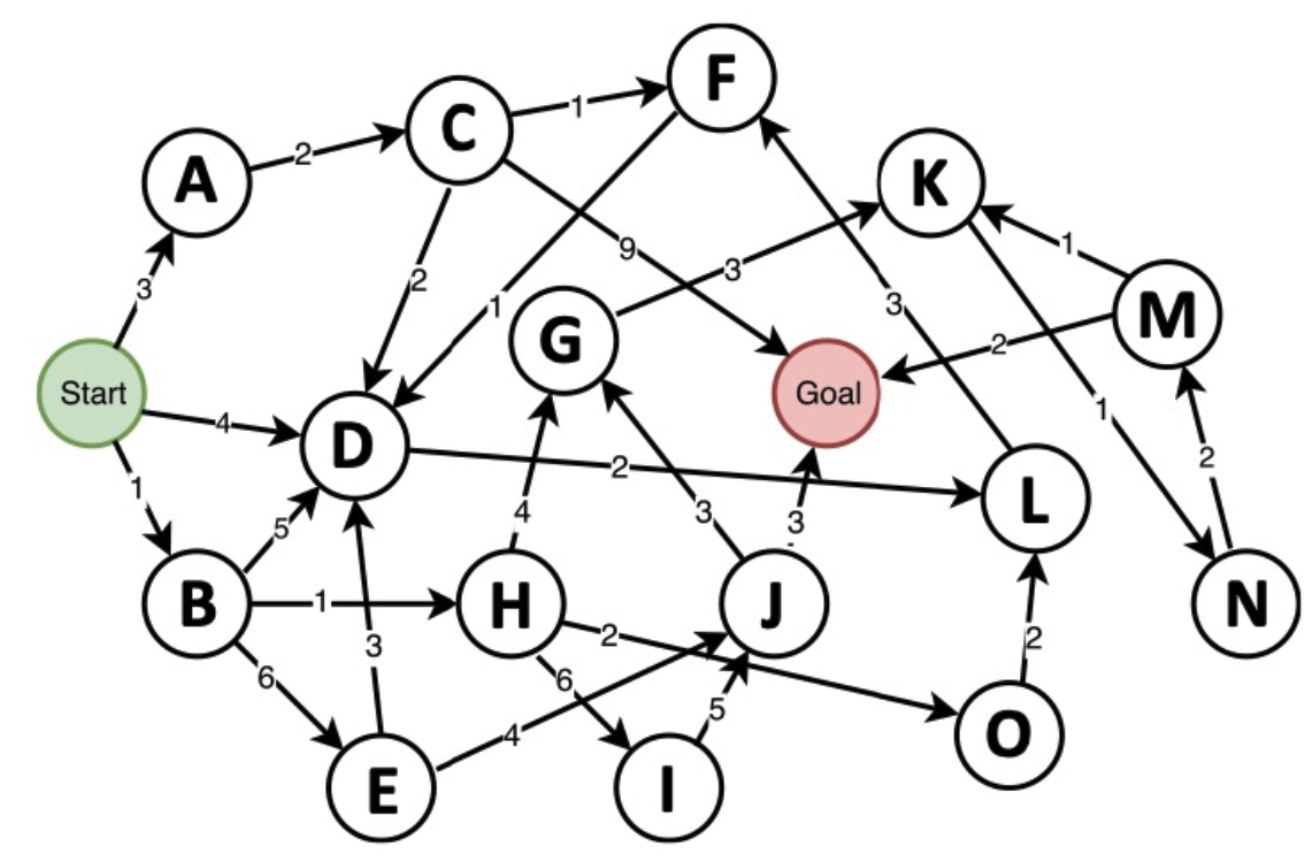
\includegraphics[width=1\linewidth]{img4.jpeg}
        \caption{More complex graph}
        \label{4}
    \end{figure}
        \subsection{Question4.1}
        Find a path form the ”start”-node to the ”goal”-node using the Dijkstra algorithm. Explain each step.

        \begin{table}[H]
            \begin{tabular}{l|l|l}
            Expanded                            & Queue                                                  & Explanation                                                \\ \hline
            Start                               & A(Start,3), \textcolor[rgb]{0,1,1}{B(Start,1)}, D(Start,4)  & Explore A and B from Start                                 \\ \hline
            Start$\rightarrow$\textcolor[rgb]{0,1,0}{B}                             & A(Start,3), D(Start,4), E(B,7), \textcolor[rgb]{0,0,1}{H(B,2)}                 & \makecell*[c]{Add B(shortest) to the queue\\ and explore DEH from B}        \\ \hline
            Start$\rightarrow$B$\rightarrow$\textcolor[rgb]{0,0,1}{H}                           & \textcolor[rgb]{1,0,0}{A(Start,3)}, D(Start,4), E(B,7), G(H,6), I(H,8), O(H,4) & \makecell*[c]{Add H(shortest) to the queue\\ and explore GIO from H}        \\ \hline
            \makecell*[c]{Start$\rightarrow$B$\rightarrow$H\\$\rightarrow$\textcolor[rgb]{1,0,0}{A}}                         & D(Start,4), E(B,7), G(H,6), I(H,8), O(H,4),C(A,5)      & \makecell*[c]{Add A(shortest) to the queue\\ and explore C from A}          \\ \hline
            \makecell*[c]{Start$\rightarrow$B$\rightarrow$H\\$\rightarrow$A$\rightarrow$O}                       & D(Start,4), E(B,7), G(H,6), I(H,8), L(O,6),C(A,5)      & \makecell*[c]{Add O(shortest) to the queue\\ and explore L from O}          \\ \hline
            \makecell*[c]{Start$\rightarrow$B$\rightarrow$H\\$\rightarrow$A$\rightarrow$O$\rightarrow$D}                     & E(B,7), G(H,6), I(H,8), L(O,6), \textcolor[rgb]{1,0,0}{C(A,5)},                & \makecell*[c]{Add D(shortest) to the queue\\ and no exploration from D}     \\ \hline
            \makecell*[c]{Start$\rightarrow$B$\rightarrow$H\\$\rightarrow$A$\rightarrow$O$\rightarrow$D\\$\rightarrow$\textcolor[rgb]{1,0,0}{C}}                   & \textcolor[rgb]{0,1,0}{E(B,7)}, G(H,6), I(H,8), L(O,6), Goal(C,14), F(C,6)     & \makecell*[c]{Add C(shortest) to the queue\\ and explore F and Goal from C} \\ \hline
            \makecell*[c]{Start$\rightarrow$B$\rightarrow$H\\$\rightarrow$A$\rightarrow$O$\rightarrow$D\\$\rightarrow$C$\rightarrow$\textcolor[rgb]{0,1,0}{E}}                 & \textcolor[rgb]{0,0,1}{G(H,6)}, I(H,8), L(O,6), Goal(C,14), F(C,6), J(E,11)    & \makecell*[c]{Add E(shortest) to the queue\\ and explore J and Goal from E} \\ \hline
            \makecell*[c]{Start$\rightarrow$B$\rightarrow$H\\$\rightarrow$A$\rightarrow$O$\rightarrow$D\\$\rightarrow$C$\rightarrow$E$\rightarrow$\textcolor[rgb]{0,0,1}{G}}               & I(H,8), L(O,6), Goal(C,14), F(C,6), J(E,11), K(G,9)    & \makecell*[c]{Add G(shortest) to the queue\\ and explore K and Goal from G} \\ \hline
            \makecell*[c]{Start$\rightarrow$B$\rightarrow$H\\$\rightarrow$A$\rightarrow$O$\rightarrow$D\\$\rightarrow$C$\rightarrow$E$\rightarrow$G\\$\rightarrow$F}             & I(H,8), L(O,6), Goal(C,14), J(E,11), K(G,9)            & \makecell*[c]{Add F(shortest) to the queue\\ and no exploration from F}     \\ \hline
            \makecell*[c]{Start$\rightarrow$B$\rightarrow$H\\$\rightarrow$A$\rightarrow$O$\rightarrow$D\\$\rightarrow$C$\rightarrow$E$\rightarrow$G\\$\rightarrow$F$\rightarrow$L}           & I(H,8), Goal(C,14), J(E,11), K(G,9)                    & \makecell*[c]{Add L(shortest) to the queue\\ and no exploration from L}     \\ \hline
            \makecell*[c]{Start$\rightarrow$B$\rightarrow$H\\$\rightarrow$A$\rightarrow$O$\rightarrow$D\\$\rightarrow$C$\rightarrow$E$\rightarrow$G\\$\rightarrow$F$\rightarrow$L$\rightarrow$I}         & Goal(C,14), J(E,11), \textcolor[rgb]{0,0,1}{K(G,9)}                            & \makecell*[c]{Add I(shortest) to the queue\\ and no exploration from I}     \\ \hline
            \makecell*[c]{Start$\rightarrow$B$\rightarrow$H\\$\rightarrow$A$\rightarrow$O$\rightarrow$D\\$\rightarrow$C$\rightarrow$E$\rightarrow$G\\$\rightarrow$F$\rightarrow$L$\rightarrow$I\\$\rightarrow$\textcolor[rgb]{0,0,1}{K}}       & Goal(C,14), \textcolor[rgb]{0,1,0}{J(E,11)}, \textcolor[rgb]{0,0,1}{N(K,10)}                           & \makecell*[c]{Add K(shortest) to the queue\\ and explore N from K}          \\ \hline
            \makecell*[c]{Start$\rightarrow$B$\rightarrow$H\\$\rightarrow$A$\rightarrow$O$\rightarrow$D\\$\rightarrow$C$\rightarrow$E$\rightarrow$G\\$\rightarrow$F$\rightarrow$L$\rightarrow$I\\$\rightarrow$K$\rightarrow$\textcolor[rgb]{0,0,1}{N}}     & Goal(C,14), \textcolor[rgb]{0,1,0}{J(E,11)}, M(N,12)                           & \makecell*[c]{Add N(shortest) to the queue\\ and explore M from N }         \\ \hline
            \makecell*[c]{Start$\rightarrow$B$\rightarrow$H\\$\rightarrow$A$\rightarrow$O$\rightarrow$D\\$\rightarrow$C$\rightarrow$E$\rightarrow$G\\$\rightarrow$F$\rightarrow$L$\rightarrow$I\\$\rightarrow$K$\rightarrow$N$\rightarrow$\textcolor[rgb]{0,1,0}{J}}   & Goal(C,14), Goal(J,14), \textcolor[rgb]{0,0,1}{M(N,12)}                        & \makecell*[c]{Add J(shortest) to the queue\\ and explore Goal from J}       \\ \hline
            \makecell*[c]{Start$\rightarrow$B$\rightarrow$H\\$\rightarrow$A$\rightarrow$O$\rightarrow$D\\$\rightarrow$C$\rightarrow$E$\rightarrow$G\\$\rightarrow$F$\rightarrow$L$\rightarrow$I\\$\rightarrow$K$\rightarrow$N$\rightarrow$J$\rightarrow$\textcolor[rgb]{0,0,1}{M}} & \textcolor[rgb]{1,0,0}{Goal(C,14)}, \textcolor[rgb]{0,1,0}{Goal(J,14)}, \textcolor[rgb]{0,0,1}{Goal(M,14)}                     & \makecell*[c]{Add M(shortest) to the queue\\ and explore Goal from M}      
            \end{tabular}
            \caption{The step of Dijkstra method}
            \end{table}
            So we can get three shortest paths: 
            \begin{itemize}
                \item Start$\rightarrow$B$\rightarrow$E$\rightarrow$J$\rightarrow$Goal, 
                \item Start$\rightarrow$B$\rightarrow$H$\rightarrow$G$\rightarrow$K$\rightarrow$N$\rightarrow$M$\rightarrow$Goal, 
                \item Start$\rightarrow$A$\rightarrow$C$\rightarrow$Goal. 
            \end{itemize} 
            The cost of the three paths are 14, 14, 14 respectively.
        \subsection{Question4.2}
        \begin{figure}[H]
            \centering
            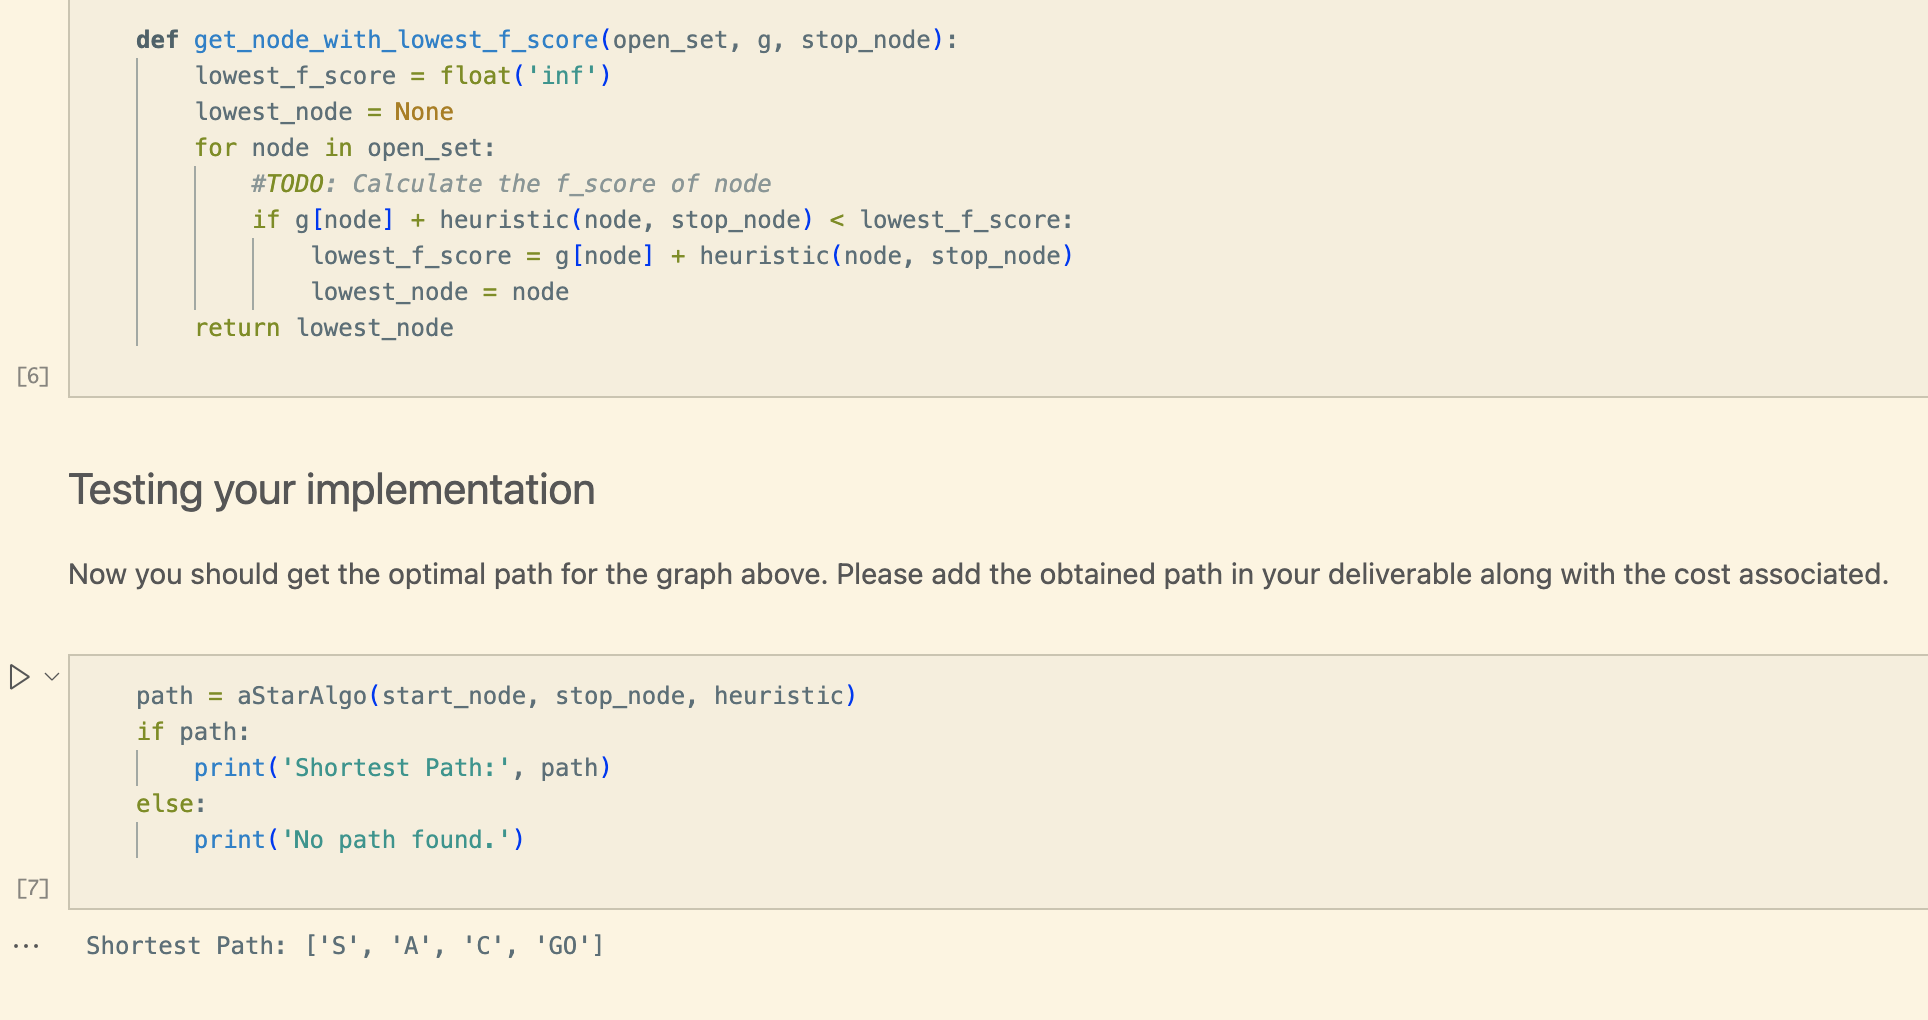
\includegraphics[width=1\linewidth]{img5.jpeg}
            \caption{The result of code implementation}
            \label{5}
        \end{figure}

    \newpage

\end{document}
